\documentclass[mathserif]{beamer} % " mathserif " option for
\usepackage{beamerthemeshadow}
\usepackage{overpic}
\usepackage{amsmath}
\usepackage{amssymb}
\usepackage{graphicx}
\usepackage{pgf}
\addtobeamertemplate{navigation symbols}{}{%
    \usebeamerfont{footline}%
    \usebeamercolor[fg]{footline}%
    \hspace{1em}%
    \insertframenumber/\inserttotalframenumber
}

\beamertemplatenavigationsymbolsempty
\setbeamertemplate{theorems}[numbered]
\newcommand{\LD}{\langle}
\newcommand{\RD}{\rangle}
\newcommand{\norm}[1]{\left\lVert #1 \right\rVert}
\newcommand{\grad}{\triangledown}
\newcommand{\R}{\mathbb{R}}
\newcommand\scalemath[2]{\scalebox{#1}{\mbox{\ensuremath{\displaystyle #2}}}}
\graphicspath{ {images/} }
\setbeamercovered{transparent}



\begin{document}


%\title{Spectral Stability of Ideal-Gas Shock Layers in the Strong Shock Limit}
\title{Finite Element MHD Solver using deal.II}
\author{Bryn Barker}%, \\ Blake Barker, Olivier Lafitte}
\date{May 4, 2021}

\setbeamercovered{invisible}
\maketitle

\begin{frame}
    \frametitle{Outline}
    \begin{itemize}
        \item[1] Motivation
        \item[2] Maxwell solver
        \item[3] Navier-Stokes solver
        \item[4] Coupled MHD solver
    \end{itemize}
\end{frame}

\begin{frame}
    \frametitle{Magnetohydrodynamics}
    MHD descirbes behavior of conducting fluids by coupling
    \begin{itemize}
\item[-] Navier-Stoke equations for fluid dynamics with
\item[-] Maxwell's equation of electromagnetism.
    \end{itemize}
    \pause

    \vskip .3cm
    MHD has applications in developing tokamak nuclear fusion reactor for power generation.
\begin{figure}
    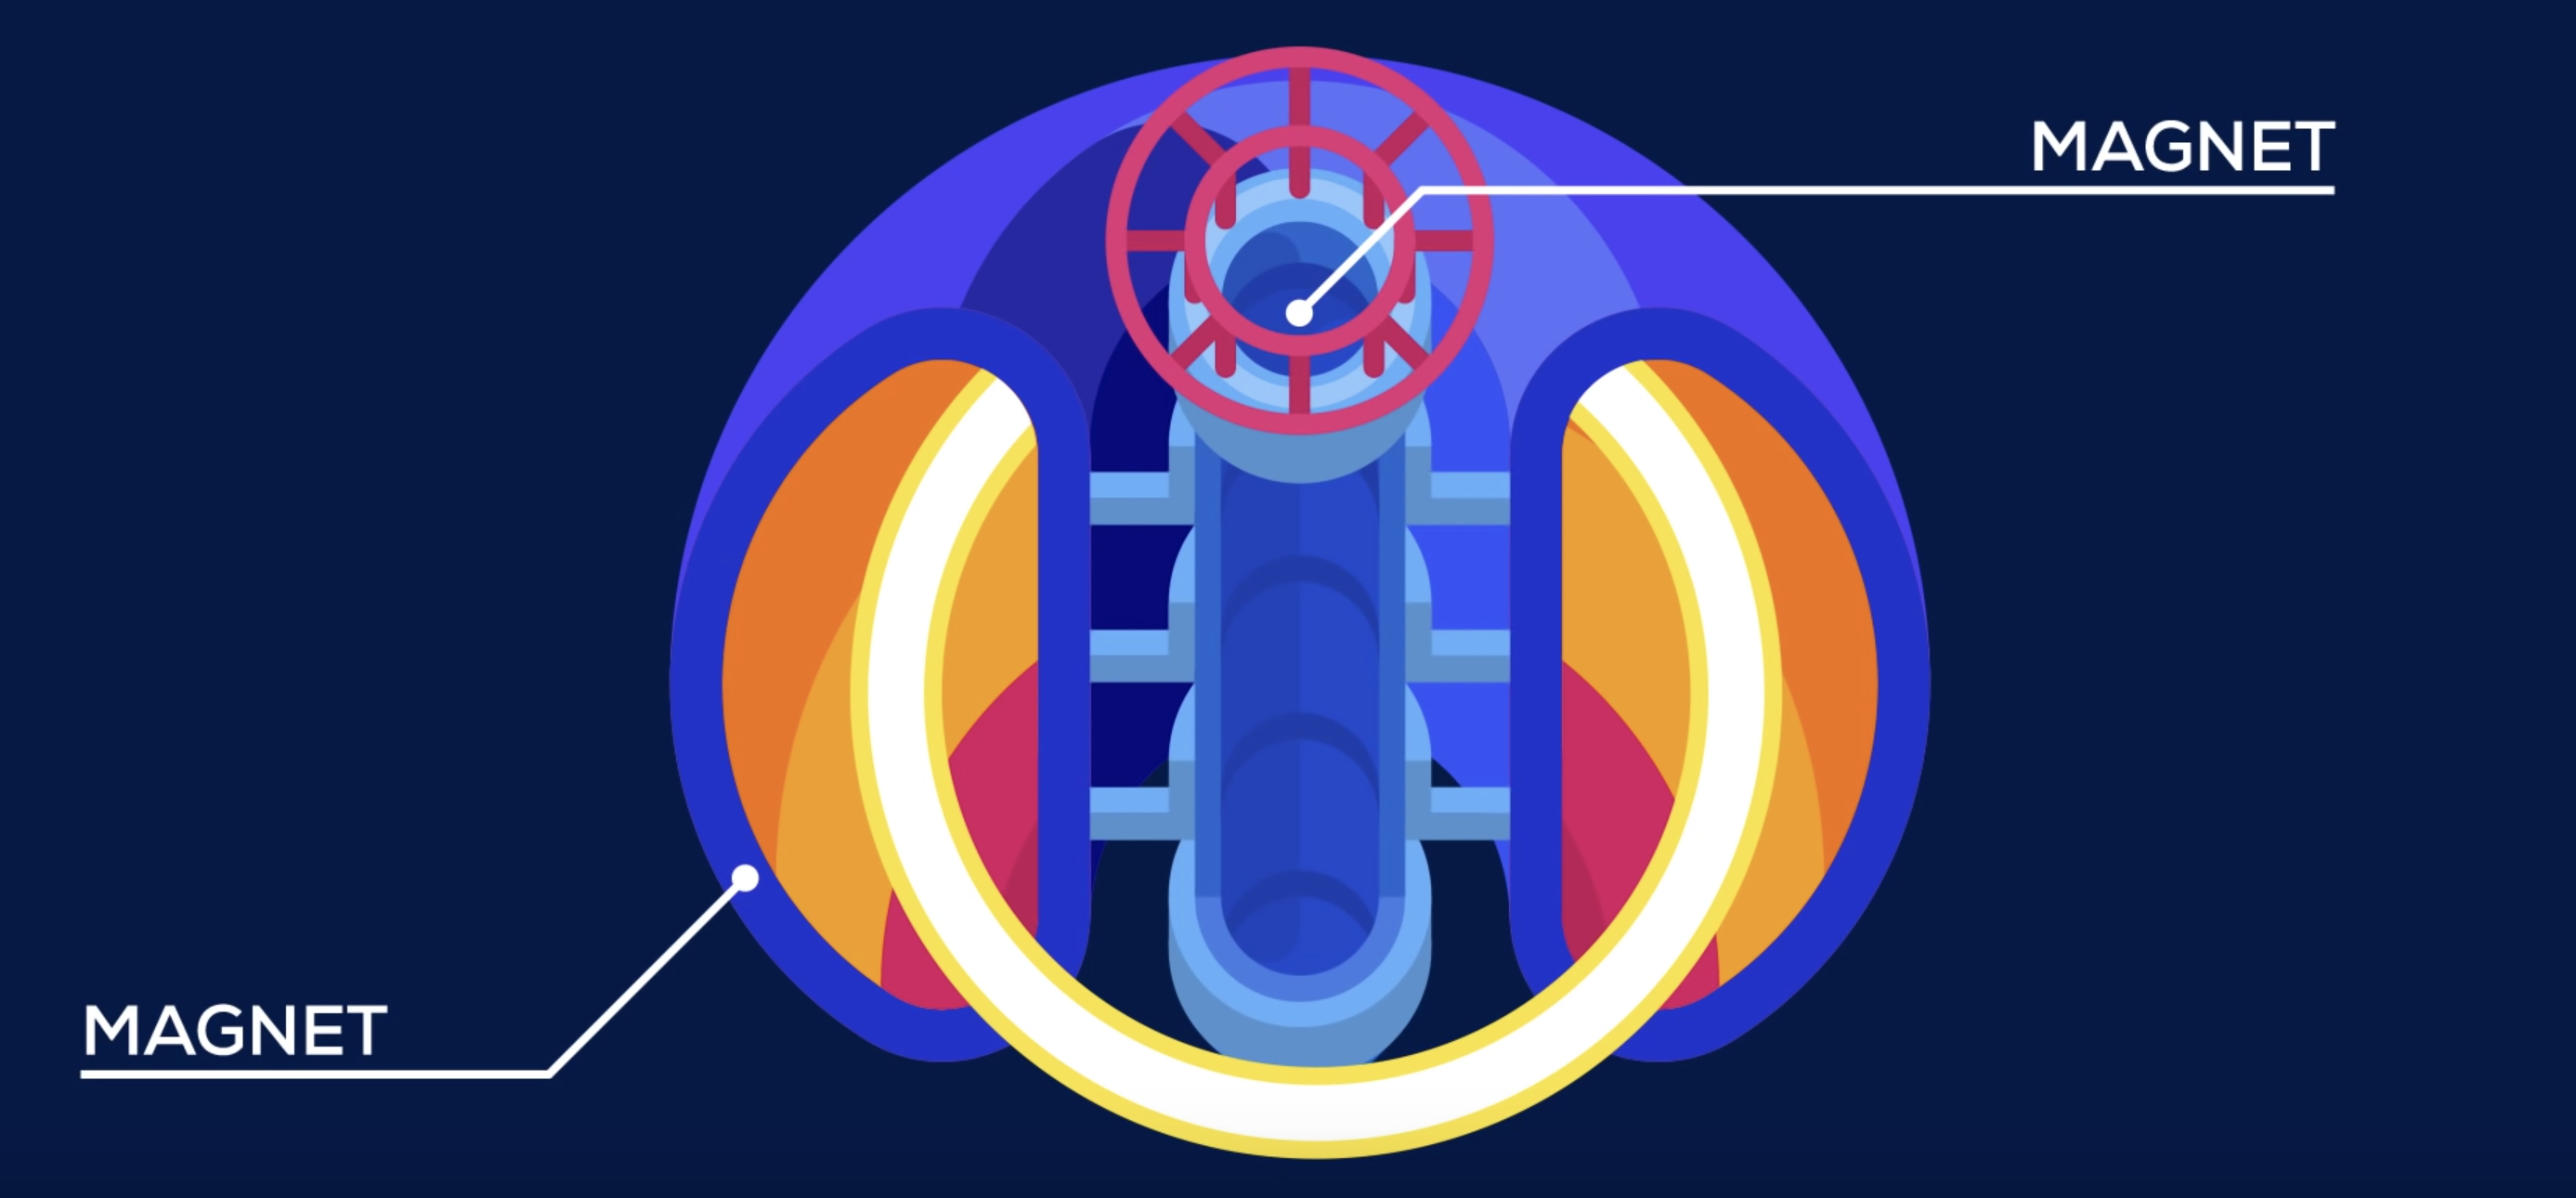
\includegraphics[width=8cm]{tokamak}
\end{figure}
\end{frame}

\begin{frame}
    \frametitle{Magnetohydrodynamics}
Equations for 2-D MHD in Eulerian Coordinates:
%\begin{subequations}
\begin{align*}
    \rho_t + \mathrm{div}(\rho u) &= 0,\nonumber\\
    (\rho u)_t + \mathrm{div}(\rho u \otimes u-h\otimes h)+\nabla q &= \mu \Delta u + (\eta + \mu) \nabla \mathrm{div} u ,\nonumber\\
    h_t - \nabla \times(u\times h)&= \nu \Delta h ,\\
(\rho E + \frac{1}{2}h^2)_t + \textrm{div}(A)&=\textrm{div}\left(\sum u\right)+\kappa \Delta T + \nu \ \textrm{div}(B),\nonumber\\
    \textrm{div}(h) &= 0,\nonumber 
\end{align*}
%\end{subequations}
\noindent 
%pressure: $p=p(\rho,T)$, specific volume: $\rho$, temperature: $T$, velocity: $u = (u_1, u_2,0)$, magnetic field: $h = (h_1, h_2,0)$, specific energy: $e$, total energy: 
%$E:= e+u_1^2/2+u_2^2/2$, $q = p + \frac{|h|^2}{2}$, 
where $ \sum:= \eta \mathrm{div}(u)I+\mu(\nabla u+(\nabla u)^t)$, $A = (\rho E+p)u+h\times(u\times h)$, $B= h\times(\grad \times h)$, $E:= e+u_1^2/2+u_2^2/2$, and $q = p + \frac{|h|^2}{2}$; see \cite{Ba,C,Da,J,Kaw}. %

%viscosity coefficients: $\mu$, $\eta$, heat conductivity coefficient: $\kappa$.
%In addition, 
%$ \sum:= \eta \mathrm{div}(u)I+\mu(\nabla u+(\nabla u)^t)$, $A = (\rho E+p)u+h\times(u\times h)$, and $B= h\times(\grad \times h)$; see %\cite{Ba,J,C,Kaw,Da}. %
%Here, $t$ is time and $(x_{1},x_2 ,x_3)$ is spatial location. Because we are only considering 2-D MHD, the solution is independent of $x_3$.

%We consider an ideal gas, so $e(\rho,T) = c_{\nu} T$ %where $c_{\nu} > 0$ is the specific heat at constant volume coefficient, and the pressure function is given by
%and 
%$p(\rho,e) = \Gamma \rho e$,
%where $\Gamma = R/c_{\nu}$. % and $R$ is the universal gas constant; see %\cite{HLyZ2}.
\end{frame}

\begin{frame}
        \frametitle{Magnetohydrodynamics:$\beta$-Model}
%The $\beta$-model is formed by adding a multiple of $\textrm{div}(h)$ to \eqref{eq1-c}, yielding the following updated system,
        In order to guarentee consistent splitting, we use the 
        $\beta$-model of our system:
%\begin{subequations}
\begin{align*}
    \rho_t + \mathrm{div}(\rho u) &= 0,\nonumber\\
    (\rho u)_t + \mathrm{div}(\rho u \otimes u-h\otimes h)+\nabla q &= \mu \Delta u + (\eta + \mu) \nabla \mathrm{div} u ,\nonumber\\
    h_t - \nabla \times(u\times h) + \textcolor{red}{\beta \textrm{div}(h)e_1}&= \nu \Delta h ,\\
(\rho E + \frac{1}{2}h^2)_t + \textrm{div}(A)&=\textrm{div}\left(\sum u\right)+\kappa \Delta T + \nu \ \textrm{div}(B),\nonumber\\
    \textrm{div}(h) &= 0,\nonumber
\end{align*}
%\end{subequations}
where $\beta$ is a real valued parameter and $e_1 = ( 1 \quad 0 )^T$; 
    %For full proofs of the mentioned properties of the $\beta$-model, 
    see \cite{BMZ}.

\end{frame}

\begin{frame}
        \frametitle{Simplified MHD}
        Major simplifications for initial model:
        \pause
        \begin{itemize}
            \item[-] Incompressible instead of compressible.
        \pause
            \item[-] Ignoring temperature/energy.
        \pause
        \end{itemize}
%\begin{subequations}
        With these simplifications our system is given by:
\begin{align*}
    \mathrm{div}(u) &= 0,\nonumber\\
    \rho( u_t + u\cdot \nabla u) +\nabla p &= \mu \Delta u +h\cdot \nabla h - \frac{1}{2}\nabla h^2,\nonumber\\
    h_t - \nabla \times(u\times h) + \beta \textrm{div}(h)e_1&= \nu \Delta h ,\\
    \textrm{div}(h) &= 0.\nonumber
\end{align*}
%\end{subequations}


\end{frame}

\begin{frame}
    \frametitle{Maxwell's Equations}
    The Maxwell's equations relevant to MHD are given by
    \[\nabla \times \boldsymbol{h} = \mu J,\quad \nabla \cdot J=0,\quad \nabla \times E = -\frac{\partial \boldsymbol{h} }{\partial t},\quad \nabla \cdot \boldsymbol{h} = 0,\]

    where \[ J = \sigma (E + \boldsymbol{u}\times \boldsymbol{h}),\]
    and $F$ is the Lorenz force given by \[ F = J\times \boldsymbol{h}.\]
    This system can be simplified to: % the induction equation:
    \begin{align*}
        \frac{\partial \boldsymbol{h} }{\partial t} - \nabla \times (\boldsymbol{u}\times \boldsymbol{h}) &+ \nu \nabla \times (\nabla \times \boldsymbol{h}) = 0,\\
        \nabla \cdot &\boldsymbol{h} = 0.
    \end{align*}


\end{frame}

\begin{frame}
    \frametitle{Maxwell's Equations}
    This system is over determined so we add a lagrange multiplier to enforce the divergence free condition.
        \pause
    \begin{align*}
        \frac{\partial \boldsymbol{h} }{\partial t} - \nabla \times (\boldsymbol{u}\times \boldsymbol{h}) + \nu \nabla &\times (\nabla \times \boldsymbol{h}) + \nabla q + \beta (\nabla \cdot \boldsymbol{h})\boldsymbol{e}_1= \boldsymbol{f},\\
        &\nabla \cdot \boldsymbol{h} = 0,
    \end{align*}
   \pause 

    The weak form corresponding to the test function $\phi = [\boldsymbol{v}\quad w]^\top$ is given by:
   \pause 
    \begin{align*}
            \left(\boldsymbol{v},\frac{\partial \boldsymbol{h} }{\partial t}\right)_\Omega
            &-\left(\nabla \times \boldsymbol{v},\boldsymbol{u}\times \boldsymbol{h}\right)_\Omega
            + \nu\left(\nabla \times\boldsymbol{v},\nabla \times \boldsymbol{h}\right)_\Omega 
            - \left(\nabla \cdot \boldsymbol{v},q\right)_\Omega \\
            &+ \beta\left(\boldsymbol{v}, (\nabla \cdot \boldsymbol{h})\boldsymbol{e}_1\right)_\Omega
            -\left(w,\nabla  \cdot \boldsymbol{h}\right)_\Omega = (\boldsymbol{v},\boldsymbol{f})_\Omega.
        \end{align*}

\end{frame}

\begin{frame}
    \frametitle{Maxwell's Equations}
    \begin{itemize}
        \item[-] To start we will consider a constant velocity field.
        \pause
        \item[-] We need $H(\text{curl})$ conforming elements : Nedelec Element for the magnetic field.
        \pause
        \item[-] Using backward Euler, at each time step, we end up with a system of the form
            \[ \begin{bmatrix} A & B^\top \\ B & 0 \end{bmatrix} \begin{bmatrix} \boldsymbol{h} \\ q \end{bmatrix} = \begin{bmatrix} F \\ 0 \end{bmatrix}
                \]
                where $A$ is composed of the mass matrix, the velocity term, and the curl curl operator. $B$ is the divergence operator. $F$ is the right hand side. 
        \pause
            \item[-] Solve using Schur decomposition with a direct solve for $A$ and the lagrange mass matrix as the preconditioner for the Schur complement.%//outer preconditioner.
    \end{itemize}
\end{frame}

\begin{frame}
    \frametitle{Maxwell Results}
    Test problem: 
    \[ \begin{bmatrix} \boldsymbol{h} \\ q\end{bmatrix} = \begin{bmatrix} t \cos(y) \\ t \sin(y) \\ 0 \end{bmatrix}.\]
        \pause


        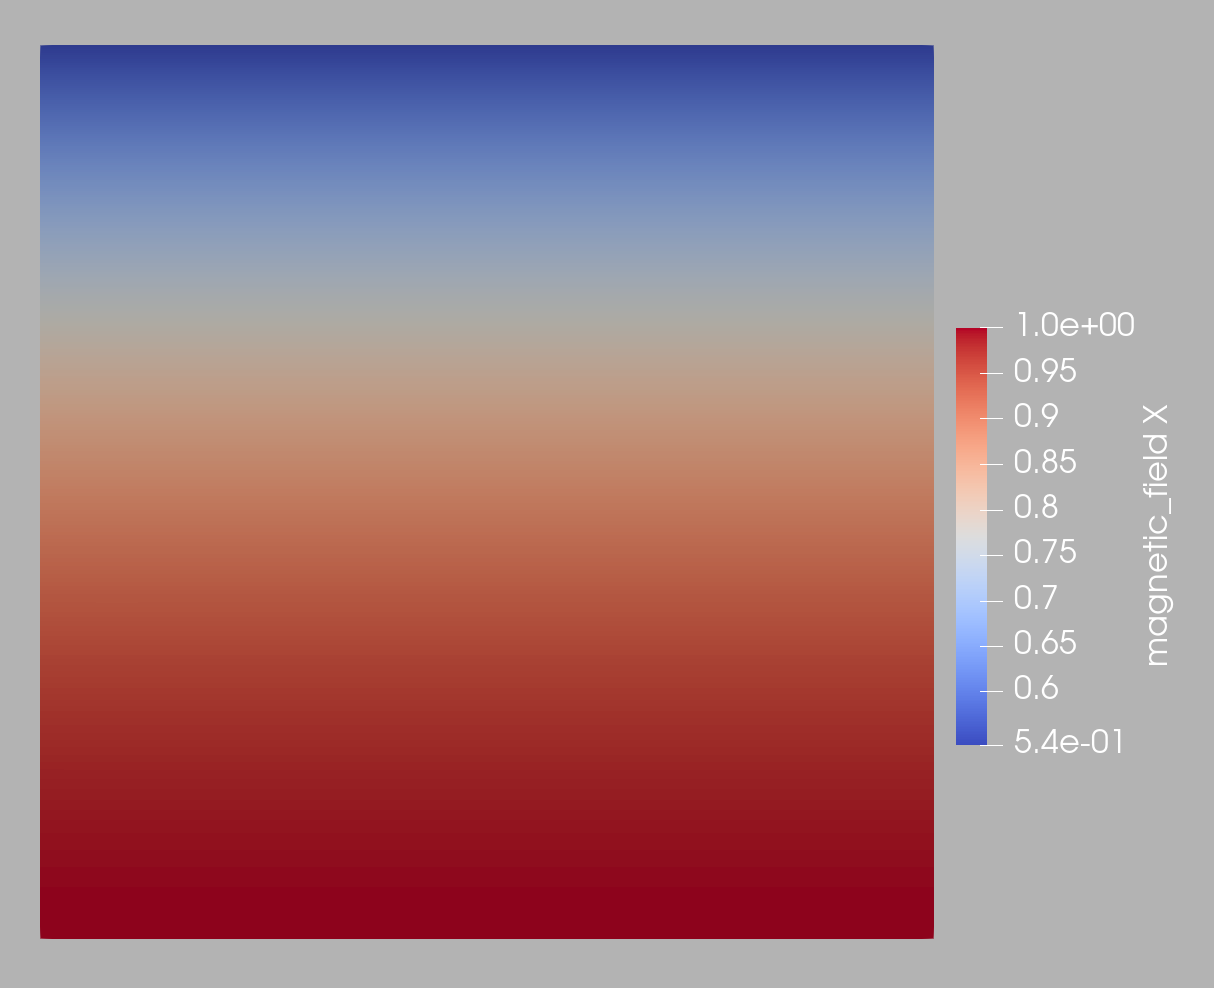
\includegraphics[width=.3\textwidth]{mag_x.png}
        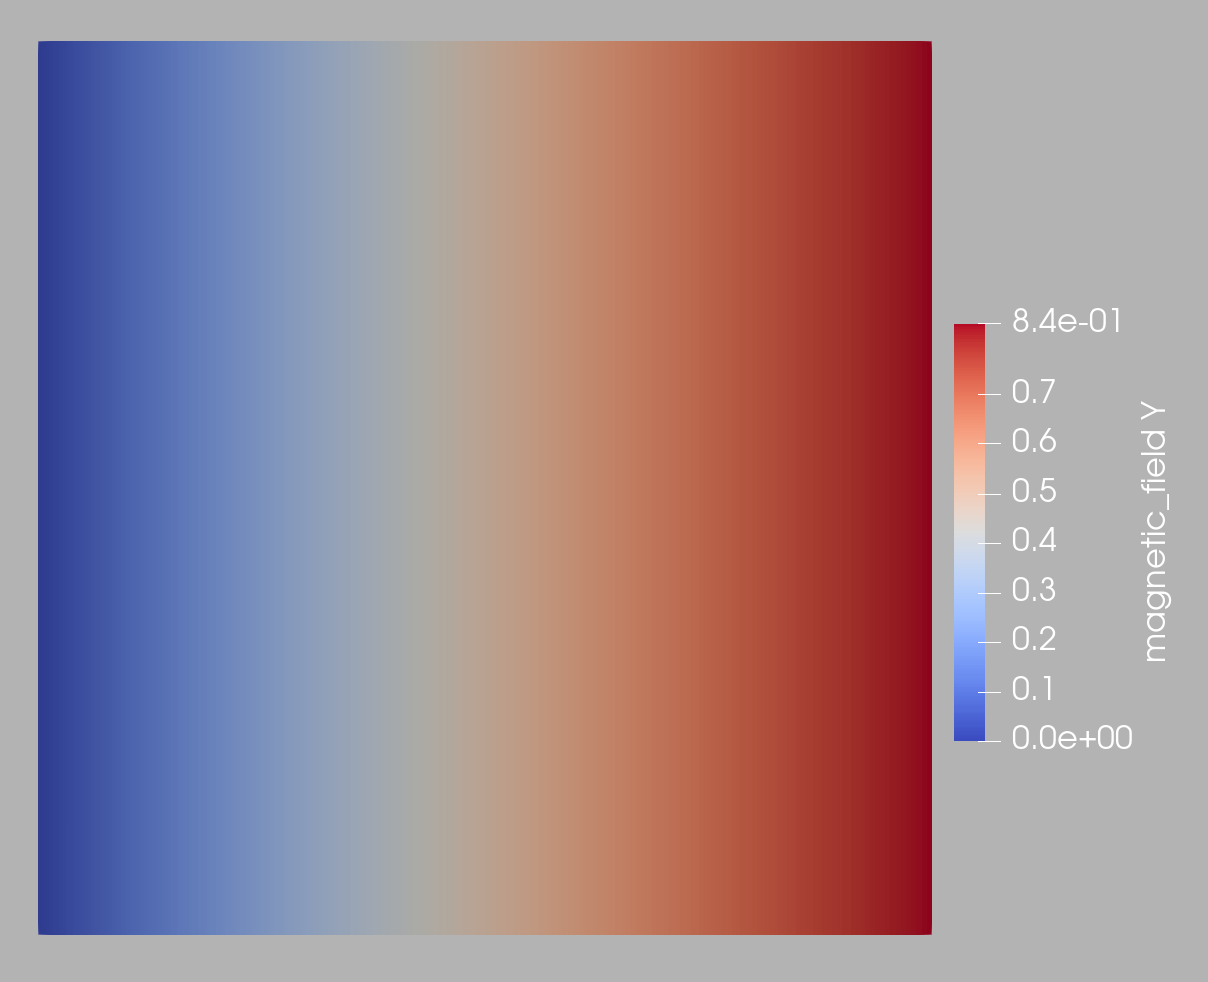
\includegraphics[width=.3\textwidth]{mag_y.png}
        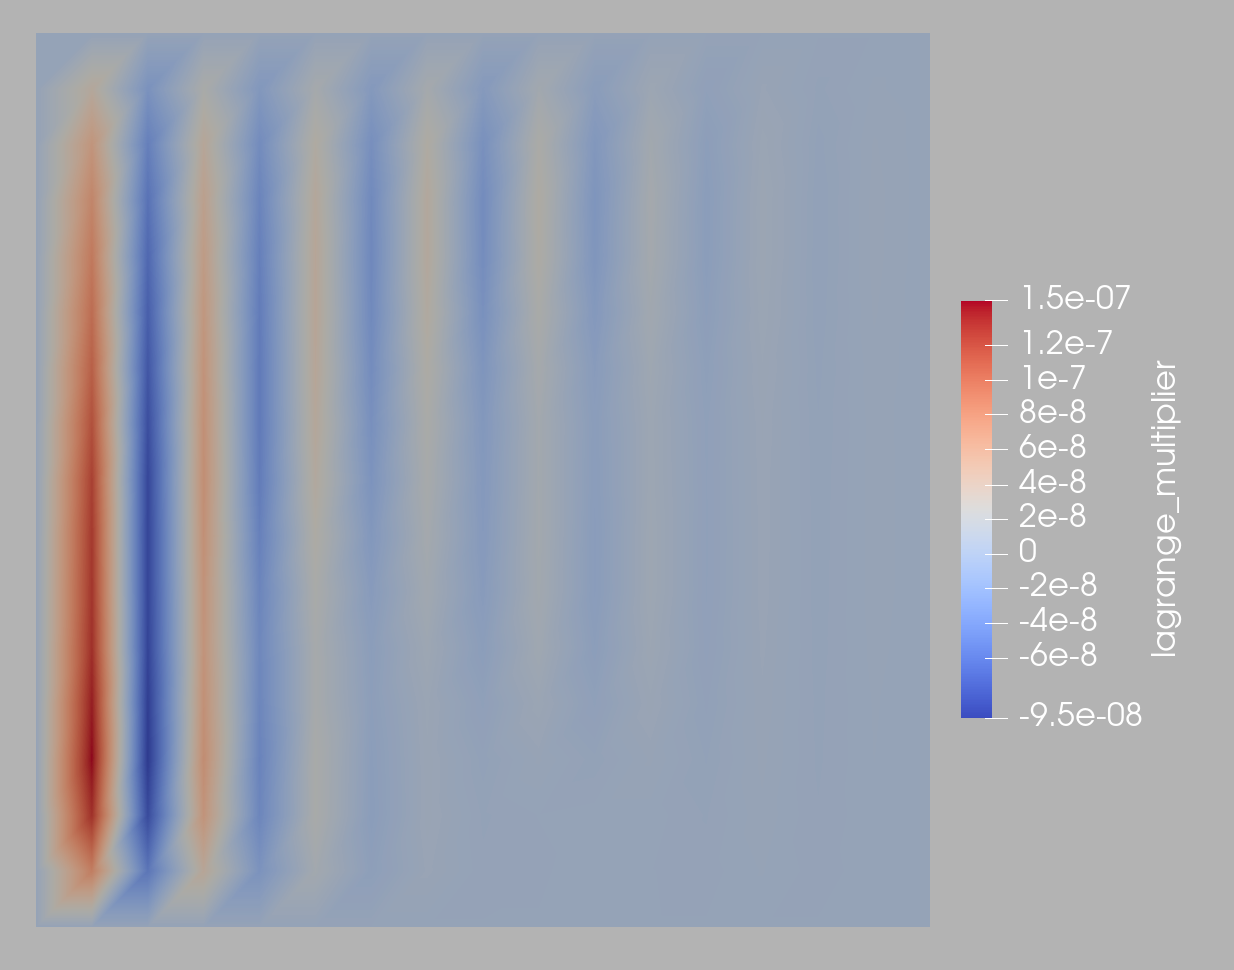
\includegraphics[width=.3\textwidth]{lagrange.png}

        Magnetic field - $x$ \hspace{.4cm} Magnetic field - $y$ \hspace{.4cm} Lagrange Multiplier
\end{frame}

\begin{frame}
    \frametitle{Maxwell Convergence}
    Second order convergence:
    \begin{center}
        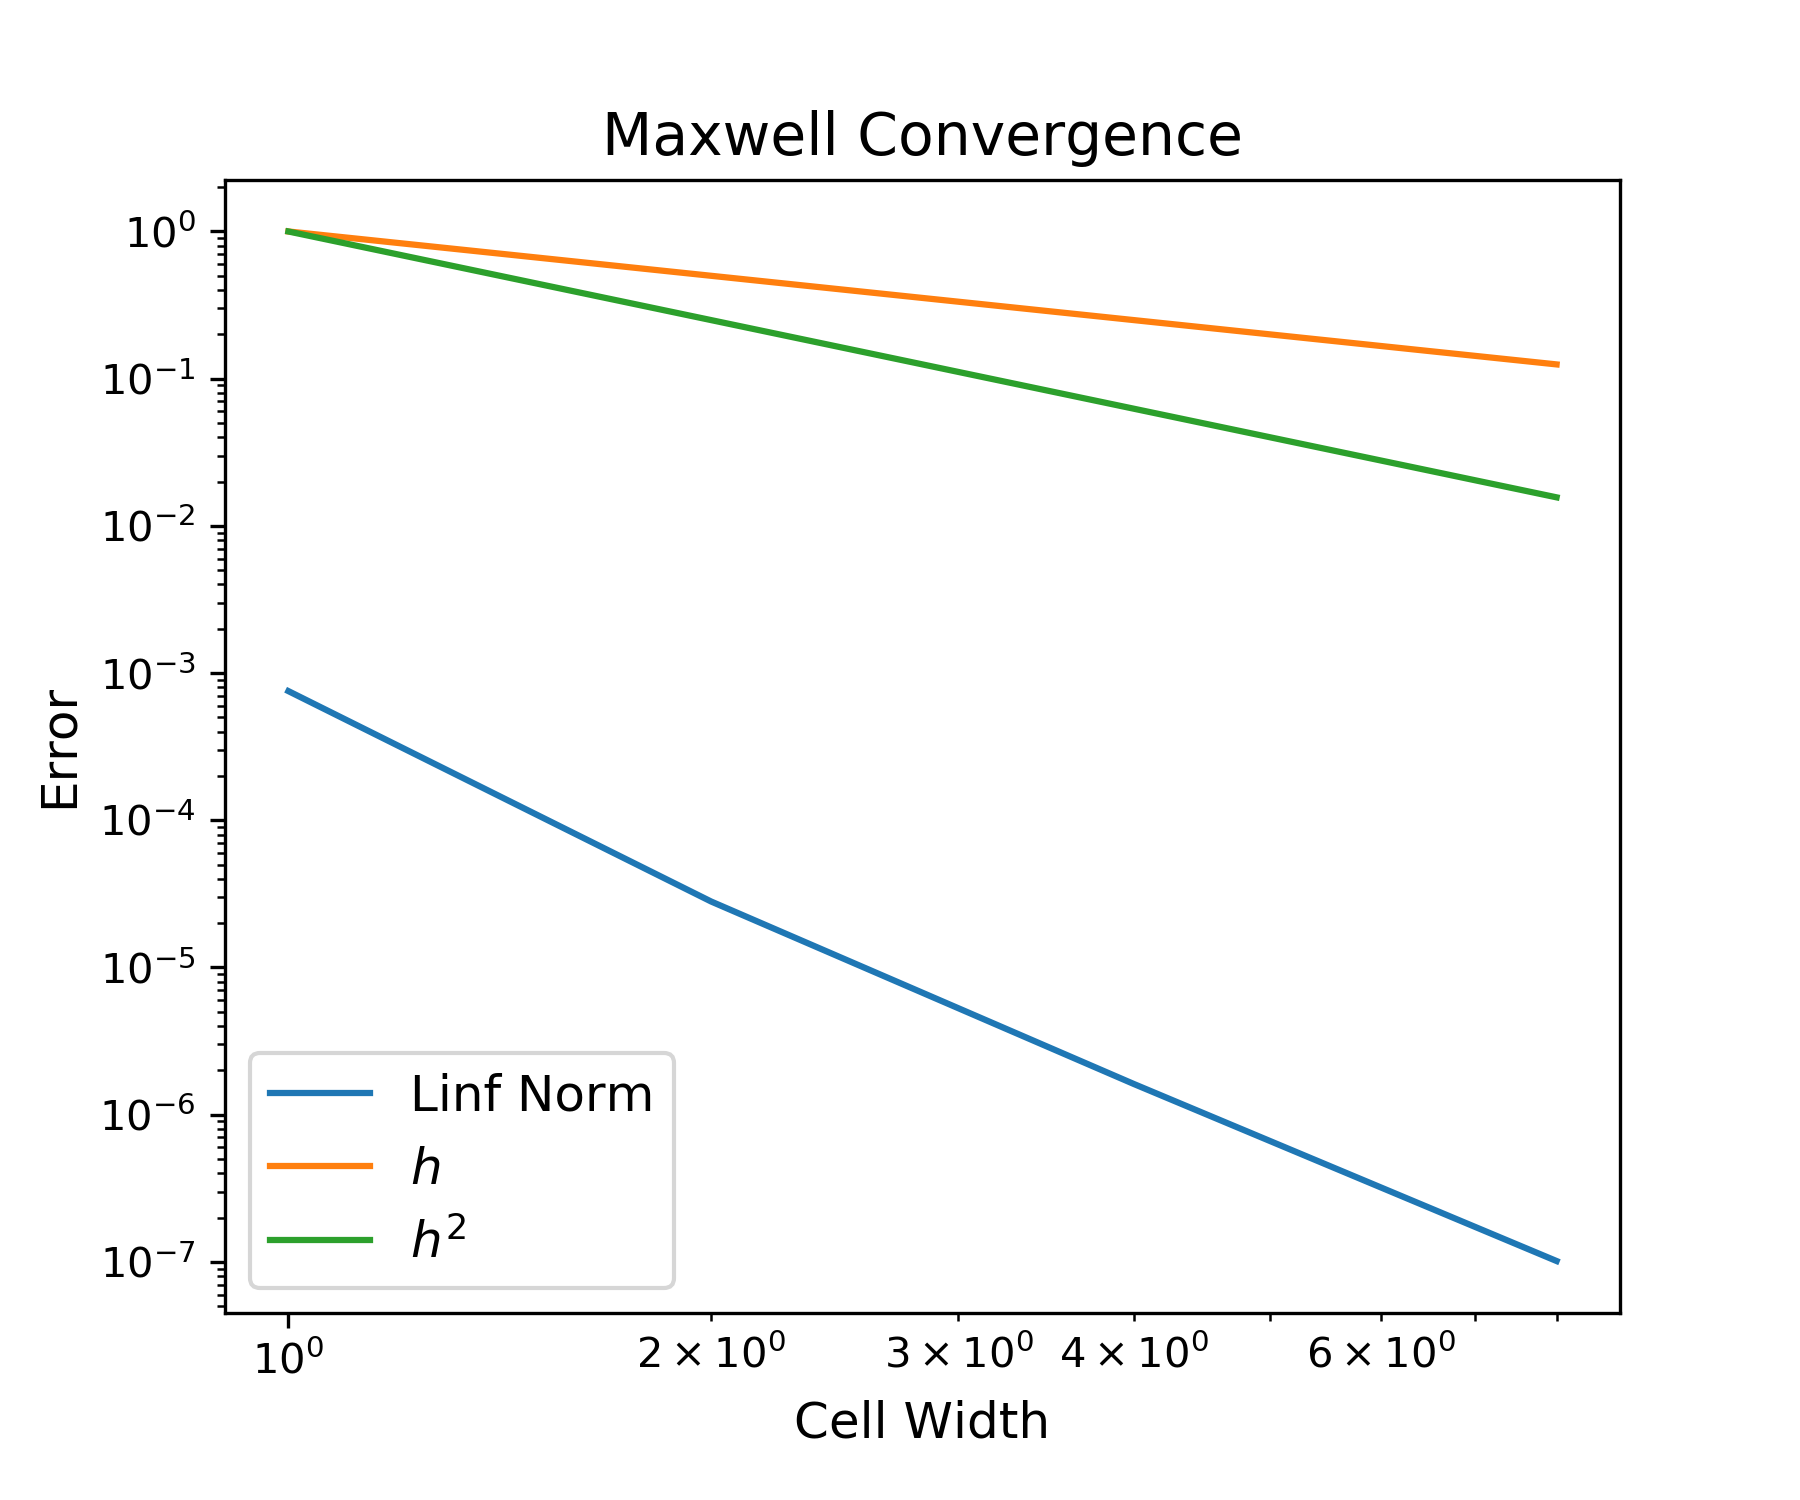
\includegraphics[scale=.5]{mx_conv.png}
    \end{center}
    Requires extremely small time step for stability.
\end{frame}

\begin{frame}
    \frametitle{Incompressible Navier-Stokes}
    Our equations for incompressible Navier-Stokes are given by:
    \begin{align*}
        -\nabla \cdot \boldsymbol{u} &= 0,\nonumber\\
        \rho \left(\frac{\partial \boldsymbol{u}}{\partial t} + \boldsymbol{u} \cdot \nabla \boldsymbol{u}\right) + \nabla p &= \mu \Delta \boldsymbol{u} + \boldsymbol{f},
    \end{align*}
    where $f$ is the Lorenz force defined using the magnetic field.

   \pause 

    \vspace{.6cm}
    This system has the following weak form:
   \pause 
    \begin{align*}
        \rho\left(\boldsymbol{v},\frac{\partial \boldsymbol{u}}{\partial t} \right)_\Omega 
        + \rho (\boldsymbol{v},\boldsymbol{u} &\cdot \nabla \boldsymbol{u})_\Omega 
        + \mu (\nabla \boldsymbol{v}, \nabla \boldsymbol{u}) _\Omega \\
        &- (\nabla \cdot \boldsymbol{v}, p) _\Omega
        - (w, \nabla \cdot \boldsymbol{u})_\Omega = (\boldsymbol{v},\boldsymbol{f})_\Omega.
    \end{align*}
\end{frame}

\begin{frame}
    \frametitle{Incompressible Navier-Stokes}
    There are a few different ways to solve this system:
        \pause
    \begin{itemize}
        \item[-] Schur decomposition with Grad-Div stabilization. This amounts to adding $\gamma \nabla (\nabla \cdot \boldsymbol{u})$ into the conservation of momentum equation and then solving similar to the Maxwell's system with different preconditioners.
        \pause
            \\
            Even with Grad-Div stabilization, the condition number of the coupled system is super bad. 
        \pause
        \item[-] Projection method, or essentially decoupling the pressure and velocity. 
    \end{itemize}
\end{frame}

\begin{frame}
    \frametitle{Navier-Stokes Results}
    Test problem: 
    \[ \begin{bmatrix} \boldsymbol{u} \\ p\end{bmatrix} = \begin{bmatrix} t \cos(y) \\ t \sin(y) \\ txy \end{bmatrix}.\]
        \pause

        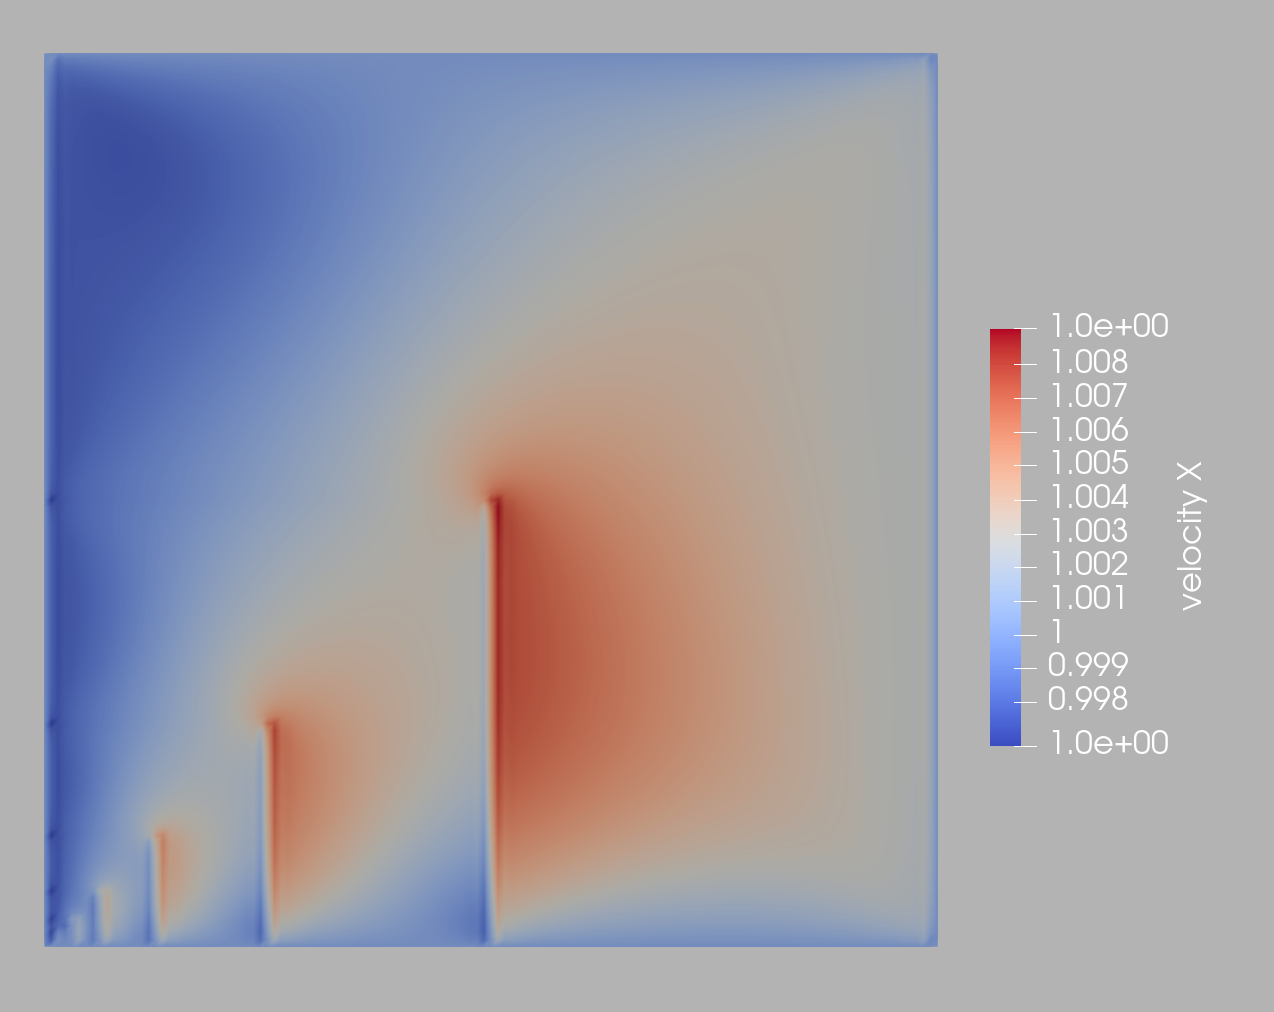
\includegraphics[width=.3\textwidth]{vel_x.png}
        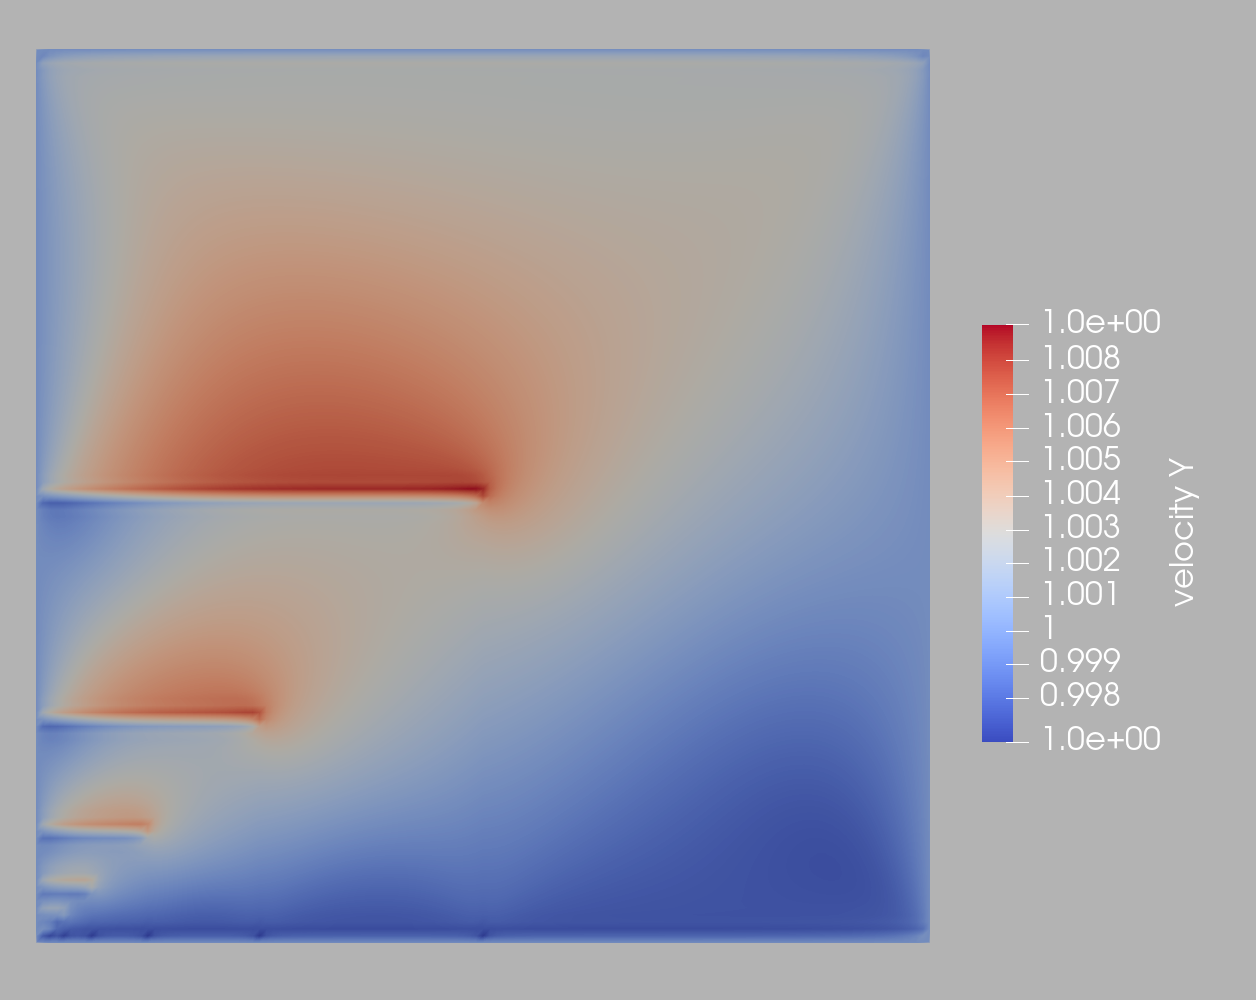
\includegraphics[width=.3\textwidth]{vel_y.png}
        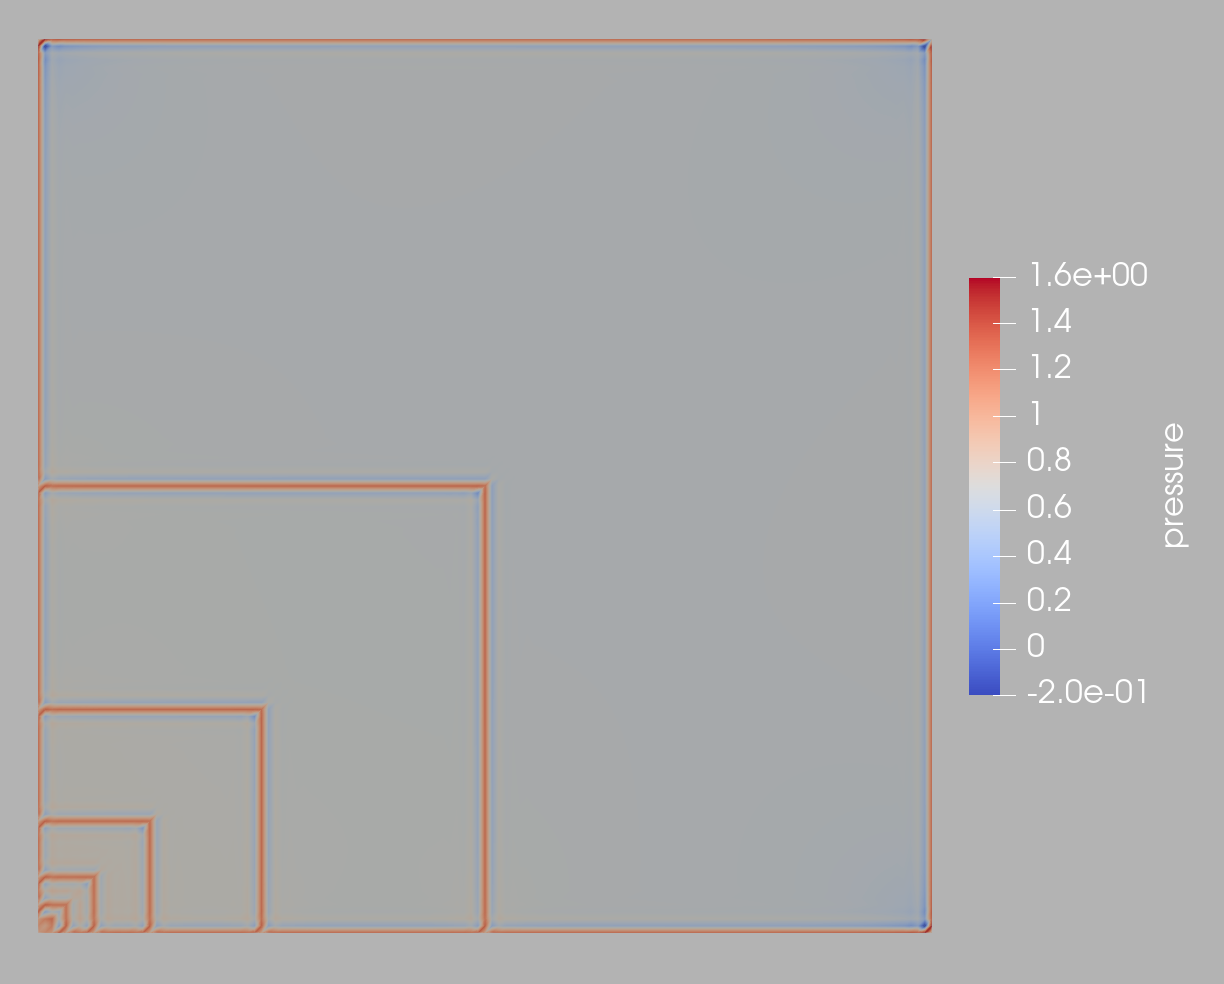
\includegraphics[width=.3\textwidth]{pressure.png}

        Velocity field - $x$ \hspace{.5cm}  Velocity field - $y$ \hspace{.5cm}  Pressure
        
        \vspace{.4cm}
        \pause

        Note: the velocity solve is what is lagging the convergence.
\end{frame}

\begin{frame}
    \frametitle{Navier-Stokes Convergence}
    First order convergence in both velocity and pressure:

    \begin{center}
        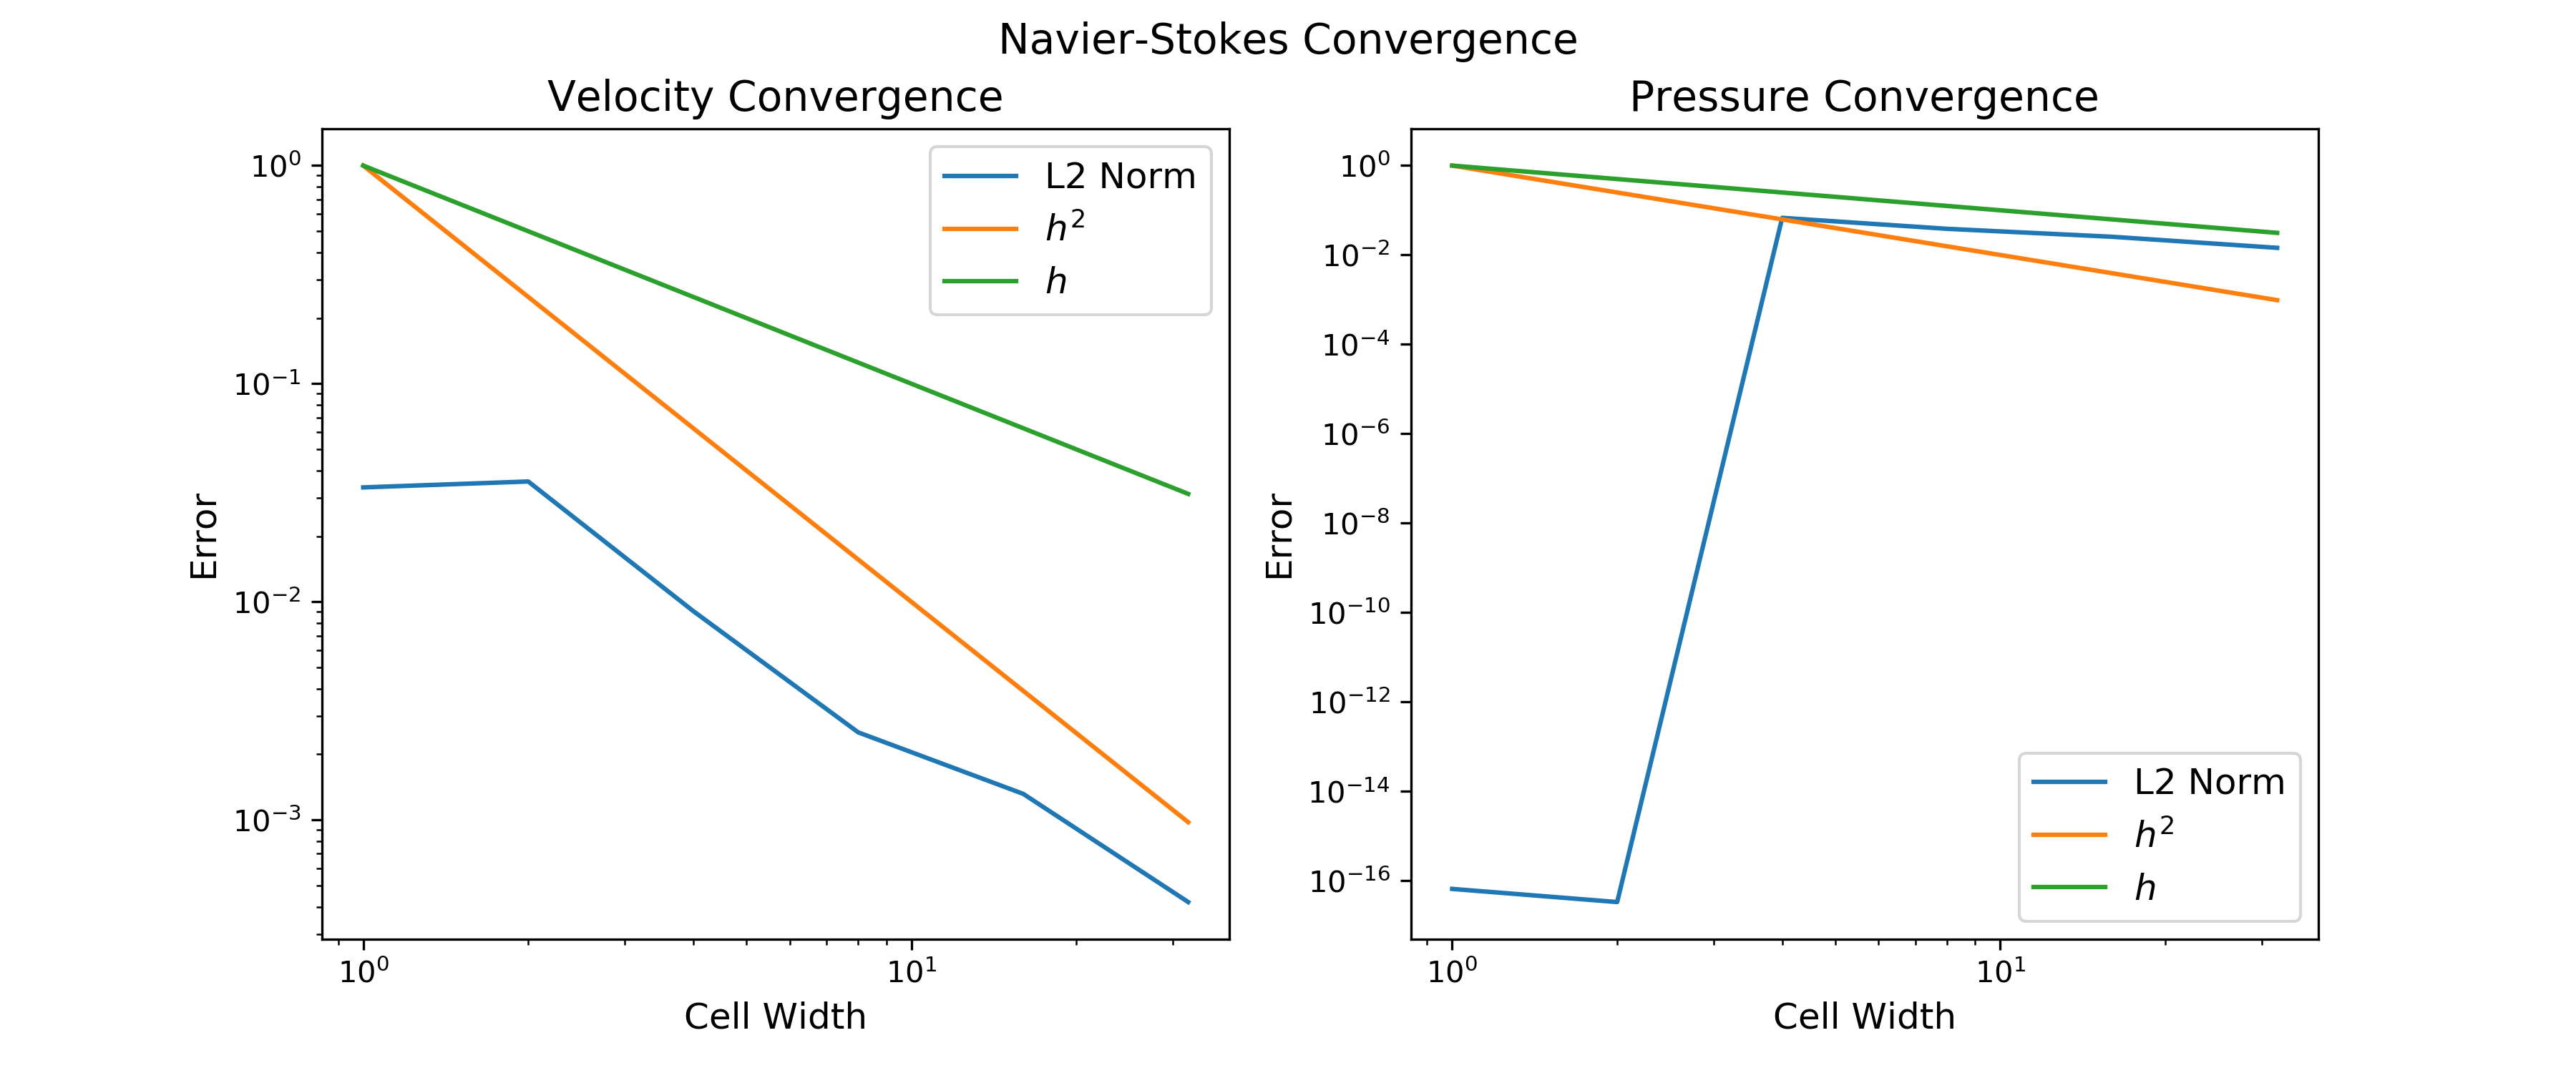
\includegraphics[scale=.35]{ns_conv.png}
    \end{center}

    Still stable with larger time step.

\end{frame}

\begin{frame}
    \frametitle{Coupling the Two Solvers}
    Our coupled system is given by:
    \begin{align*}
        \frac{\partial \boldsymbol{h} }{\partial t} - \nabla \times (\boldsymbol{u}\times \boldsymbol{h}) + \nu \nabla &\times (\nabla \times \boldsymbol{h}) + \nabla q + \beta (\nabla \cdot \boldsymbol{h})\boldsymbol{e}_1= 0,\\
        &\nabla \cdot \boldsymbol{h} = 0,\\
        \rho \left(\frac{\partial \boldsymbol{u}}{\partial t} + \boldsymbol{u} \cdot \nabla \boldsymbol{u}\right) + \nabla p &= \mu \Delta \boldsymbol{u} + \boldsymbol{h}\cdot \nabla \boldsymbol{h} - \frac{1}{2}\nabla \boldsymbol{h}^2, \\
        -&\nabla \cdot \boldsymbol{u} = 0,\nonumber
    \end{align*}
    \pause
    To start we will initialize $\boldsymbol{h}^0$, $q^0$, $\boldsymbol{u}^0$, and $p^0$ using initial conditions. 
    \pause

    And we will set $u^1 \approx u^0$ and $p^1 \approx p^0$.
\end{frame}

\begin{frame}
    \frametitle{Solving the Coupled System}
    
    Then we will solve two steps with the maxwell solver to catch up to the velocity before solving both systems in each time step.
    \pause

    \vspace{.4cm}
    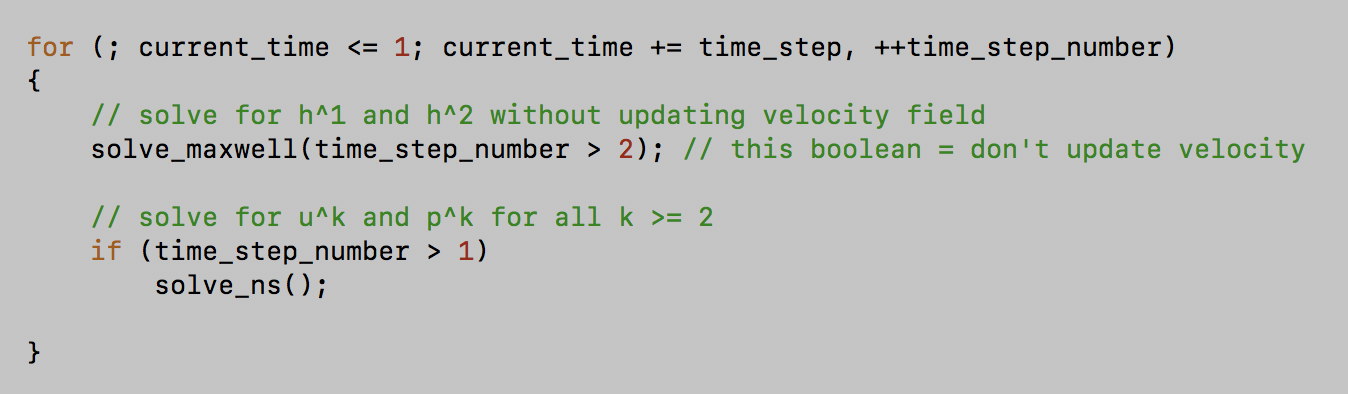
\includegraphics[scale=.45]{solver.png}
      
\end{frame}

\begin{frame}
    \frametitle{Testing the Coupled Solver}
    \begin{itemize}
            \pause
        \item[-] Method of manufactured solutions is not meaningful because the coupling occurs in the forcing term of the Navier-Stokes equations. 
            \pause
        \item[-] Need to test with exact solution.

    \vspace{.4cm}
            \pause
            To start, we test with a constant solution (constant magnetic field, velocity field, and pressure) to make sure the coupling is set-up correctly.

    \end{itemize}

\end{frame}

\begin{frame}
    \frametitle{Testing the Coupled Solver}
    Convergence results for the constant solution:

    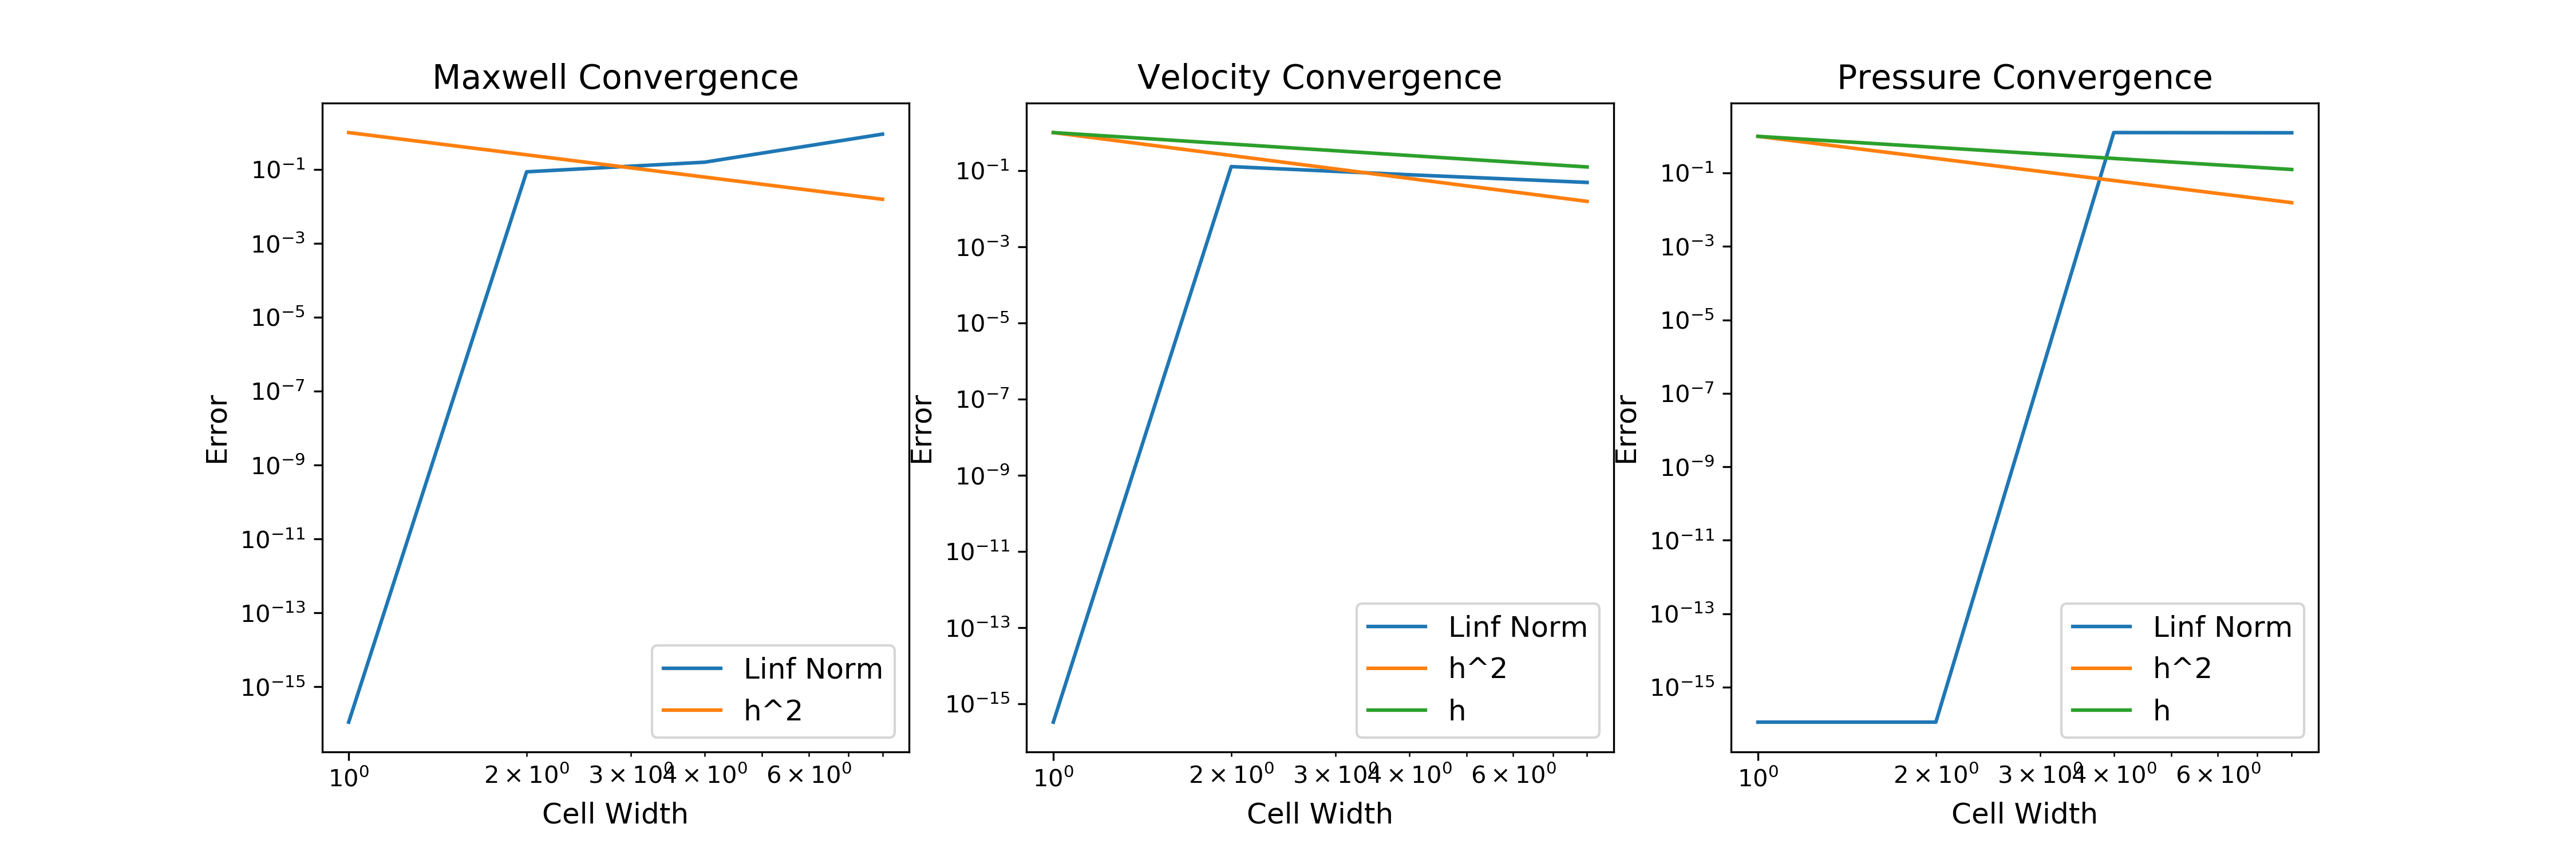
\includegraphics[scale=.3]{full_conv.png}


\end{frame}

\begin{frame}
    \frametitle{Testing the Coupled Solver}

    Identifying the weakness in the solver.

    \pause

    \begin{center}
        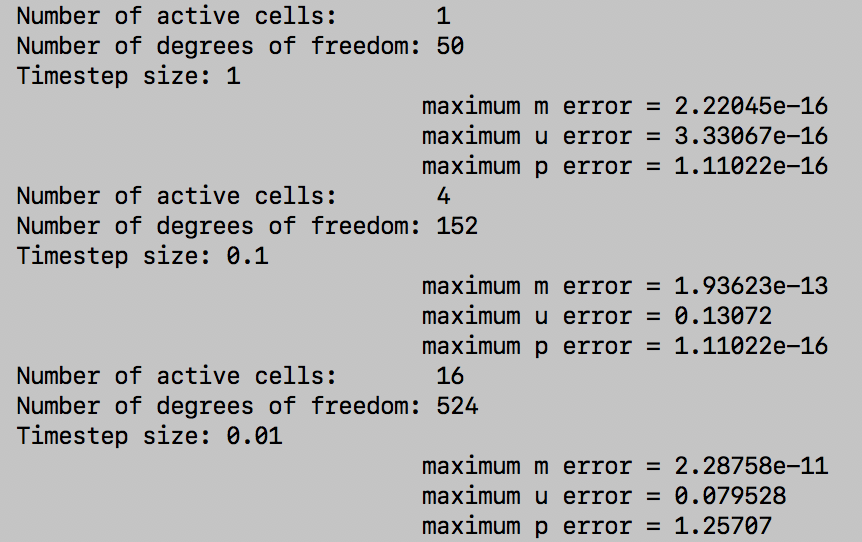
\includegraphics[width=.45\textwidth]{exact_mag.png}
        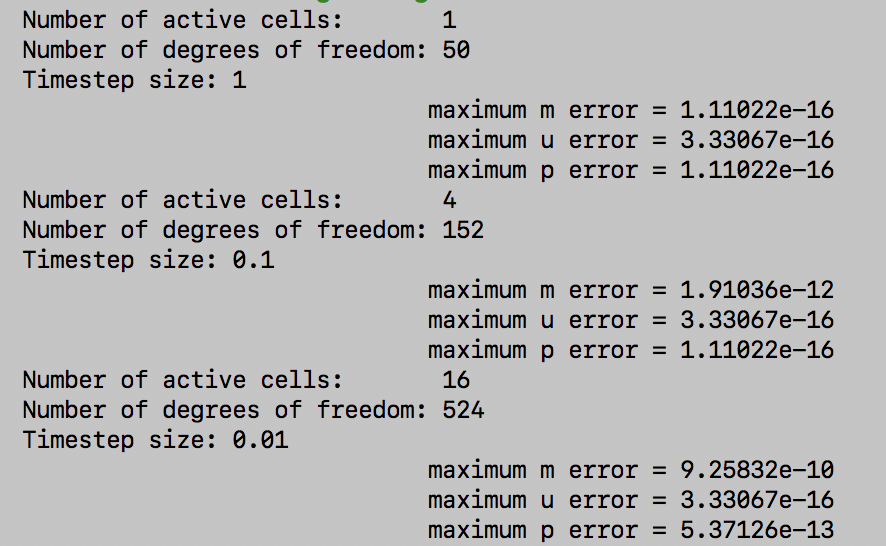
\includegraphics[width=.45\textwidth]{exact_vel.png}
    \end{center}

      \hspace{.4cm}  Exact Magnetic field \hspace{1.8cm}  Exact Velocity field

      \vfill


\end{frame}
\begin{frame}
    \frametitle{Next Steps}
    \pause
    \begin{itemize}
        \item[-] Speed up code.
            \pause
        \item[-] Improve incompressible Navier-Stokes solver.
    \pause
\item[-] Test coupled incompressible solver on harder solutions (ex. Alven wave or stationary traveling wave).
    \pause
        \item[-] Create compressible Navier-Stokes solver.
    \pause
        \item[-] Add in temperature equation.
    \pause
        \item[-] Test with traveling wave stability with stationary traveling wave.
    \end{itemize}
\end{frame}

\begin{frame}
    \frametitle{That's It!}
\end{frame}

\bibliography{refs}
\bibliographystyle{plain}
\end{document}
